\documentclass{article}

\usepackage[utf8]{inputenc}
\usepackage[T1]{fontenc}
\usepackage[spanish]{babel}
\usepackage{physics}
\usepackage{tikz}
\usetikzlibrary{babel}
\usepackage{listings}
\usepackage{graphicx}
\usepackage{subcaption}

\DeclareMathOperator{\arsinh}{arsinh}

\title{Mecánica Estadística: Tarea 4\\ Modelo de Ising - Transiciones de Fase}
\author{Iván Mauricio Burbano Aldana}

\begin{document}

\maketitle

\section{Dualidad}

\subsection{Desarrollo de baja temperatura}

1. Como las condiciones de frontera son periódicas, la red cuadrada se puede considerar como embebida en un toro. En tal caso, cada espín tiene 4 vecinos. Por lo tanto la suma de los vecinos en cada vértice de la red es $4N$. En este cálculo cada par de vecinos se cuenta dos veces, una por cada vértice en el par. Luego el número total de pares de vecinos es
\begin{equation}
s=\frac{4N}{2}=2N.
\end{equation}

2. Vemos que el término
\begin{equation}
\sigma_i\sigma_j=\begin{cases}
1 & \sigma_i=\sigma_j \\
-1 & \sigma_i\neq\sigma_j
\end{cases}
\end{equation}
pues $\sigma_i,\sigma_j\in\qty{-1,1}$. Ahora bien, podemos caracterizar $r$ como
\begin{equation}
r=|\qty{\langle i,j\rangle|\text{el espín $i$ es antiparalelo al espín $j$}}|=|\{\langle i,j\rangle|\sigma_i\neq\sigma_j\}|.
\end{equation}
De manera análoga
\begin{equation}
s-r=|\qty{\langle i,j\rangle|\text{el espín $i$ es paralelo al espín $j$}}|=|\{\langle i,j\rangle|\sigma_i=\sigma_j\}|.
\end{equation}
Luego
\begin{equation}
\sum_{\langle i,j\rangle}\sigma_i\sigma_j=1|\{\langle i,j\rangle|\sigma_i=\sigma_j\}|-1|\{\langle i,j\rangle|\sigma_i\neq\sigma_j\}|=s-r-r=s-2r.
\end{equation}

3. Se tiene una función de partición
\begin{align}
\begin{split}
Z(T)=&\sum_{(\sigma_1,\dots,\sigma_N)\in\{-1,1\}^N}e^{\beta J\sum\limits_{\langle i,j\rangle}\sigma_i\sigma_j}=\sum_{(\sigma_1,\dots,\sigma_N)\in\{-1,1\}^N}e^{L(s-2r)}\\
=&e^{Ls}\sum_{(\sigma_1,\dots,\sigma_N)\in\{-1,1\}^N}e^{-2Lr}=e^{Ls}\sum_{r=0}^s A_re^{-2Lr}
\end{split}
\end{align}
donde $A_r$ es el número de configuraciones $(\sigma_1,\dots,\sigma_N)\in\{0,1\}^N$ con $r$ pares de espines antiparalelos. Ahora bien, note que la configuración $(\sigma_1,\dots,\sigma_N)\in\{0,1\}^N$ tiene el mismo número de espines antiparalelos que $(-\sigma_1,\dots,-\sigma_N)$. Luego $A_r=2\omega_r$ donde $\omega_r$ es el numero de configuraciones $(\sigma_1,\dots,\sigma_N)\in\{0,1\}^N$ con $r$ pares de espines antiparalelos salvo multiplicación por $-1$. Luego
\begin{equation}
Z(T)=2e^{Ls}\sum_{r=0}^s\omega_re^{-2Lr}.
\end{equation}
Mas aún, las únicas configuraciones que tienen $0$ pares de espines antiparalelos son $(1,\dots,1)$ y $(-1,\dots,-1)$. Luego $\omega_0=1$ y 
\begin{equation}\label{ec:funcion_de_particion}
Z(T)=2e^{Ls}\qty(e^0+\sum_{r=1}^s\omega_re^{-2Lr})=2e^{Ls}\qty(1+\sum_{r=1}^s\omega_re^{-2Lr}).
\end{equation}

4. Note que si $T\ll J/k_B$ entonces $L=J/k_B T\gg 1$. Entonces $e^{2L}\gg 1$ y 
\begin{equation}
e^{-2L}=\frac{1}{e^{2L}}\ll 1.
\end{equation}
Luego el factor
\begin{equation}
1+\sum_{r=1}^s\omega_re^{-2Lr}=\sum_{r=0}^s\omega_r\qty(e^{-2L})^r
\end{equation}
es una expansión en serie de potencias de $e^{-2L}$ que puede ser aproximada ignorando los términos de orden superior. Es por esto que la expresión \eqref{ec:funcion_de_particion} es una desarrollo de baja temperatura de la función de partición. 

\subsection{Auto-dualidad y determinación de la temperatura crítica}

1. Ver figura \ref{fig:configuracion}.
\begin{figure}
\begin{center}
\begin{tikzpicture}
\draw [help lines] (0,0) grid (5,5);
\foreach \x in {0,...,5}
\foreach \y in {0,...,5}
{
\draw [fill] (\x,\y) circle [radius=0.06];
}
\draw [ultra thick, blue] (1, 4) -- (0,4) -- (0,5) -- (1,5) -- (1,4) -- (1, 3) -- (2, 3) -- (2,4) -- (1, 4);
\draw [ultra thick, blue] (3, 4) -- (4,4) -- (4,3) -- (5,3) -- (5,2) -- (4,2) -- (3,2) -- (3,3) -- (3, 4);
\draw [ultra thick, blue] (1, 1) -- (2,1) -- (2,2) -- (1,2) -- (1,1);
\end{tikzpicture}
\caption{\label{fig:configuracion}Un gráfico de 20 barras que contribuye sobre un retículo cuadrado de 36 vértices.}
\end{center}
\end{figure}

2. Ver figura \ref{fig:configuracion_dual}.
\begin{figure}
\begin{center}
\begin{tikzpicture}
\draw [help lines] (0,0) grid (5,5);
\draw [step = 1] (0.5,0.5) grid (4.5,4.5);
\foreach \x in {0,...,5}
\foreach \y in {0,...,5}
{
\draw [fill] (\x,\y) circle [radius=0.06];
}
\foreach \x in {0,...,4}
\foreach \y in {0,...,4}
{
\draw [help lines, dashed] (\x+0.5, 0) -- (\x+0.5, 5);
\draw [help lines, dashed] (0, \y+0.5) -- (5, \y+0.5);
}
\draw [->, ultra thick, red] (0.5, 4.2) -- (0.5, 4.8);
\draw [->, ultra thick, red] (1.5, 3.2) -- (1.5, 3.8);
\draw [->, ultra thick, red] (1.5, 1.2) -- (1.5, 1.8);
\draw [->, ultra thick, red] (3.5, 3.2) -- (3.5, 3.8);
\draw [->, ultra thick, red] (3.5, 2.2) -- (3.5, 2.8);
\draw [->, ultra thick, red] (4.5, 2.2) -- (4.5, 2.8);
\draw [->, ultra thick, red] (1.5, 4.8) -- (1.5, 4.2);
\draw [->, ultra thick, red] (2.5, 4.8) -- (2.5, 4.2);
\draw [->, ultra thick, red] (3.5, 4.8) -- (3.5, 4.2);
\draw [->, ultra thick, red] (4.5, 4.8) -- (4.5, 4.2);
\draw [->, ultra thick, red] (0.5, 3.8) -- (0.5, 3.2);
\draw [->, ultra thick, red] (2.5, 3.8) -- (2.5, 3.2);
\draw [->, ultra thick, red] (4.5, 3.8) -- (4.5, 3.2);
\draw [->, ultra thick, red] (0.5, 2.8) -- (0.5, 2.2);
\draw [->, ultra thick, red] (1.5, 2.8) -- (1.5, 2.2);
\draw [->, ultra thick, red] (2.5, 2.8) -- (2.5, 2.2);
\draw [->, ultra thick, red] (0.5, 1.8) -- (0.5, 1.2);
\draw [->, ultra thick, red] (2.5, 1.8) -- (2.5, 1.2);
\draw [->, ultra thick, red] (3.5, 1.8) -- (3.5, 1.2);
\draw [->, ultra thick, red] (4.5, 1.8) -- (4.5, 1.2);
\draw [->, ultra thick, red] (0.5, 0.8) -- (0.5, 0.2);
\draw [->, ultra thick, red] (1.5, 0.8) -- (1.5, 0.2);
\draw [->, ultra thick, red] (2.5, 0.8) -- (2.5, 0.2);
\draw [->, ultra thick, red] (3.5, 0.8) -- (3.5, 0.2);
\draw [->, ultra thick, red] (4.5, 0.8) -- (4.5, 0.2);
\draw [ultra thick, blue] (1, 4) -- (0,4) -- (0,5) -- (1,5) -- (1,4) -- (1, 3) -- (2, 3) -- (2,4) -- (1, 4);
\draw [ultra thick, blue] (3, 4) -- (4,4) -- (4,3) -- (5,3) -- (5,2) -- (4,2) -- (3,2) -- (3,3) -- (3, 4);
\draw [ultra thick, blue] (1, 1) -- (2,1) -- (2,2) -- (1,2) -- (1,1);
\end{tikzpicture}
\caption{\label{fig:configuracion_dual}En la red dual sobre la figura \ref{fig:configuracion} se dibujan espines hacia arriba dentro de los polígonos y espines hacia abajo fuera.}
\end{center}
\end{figure}

3. Note que el número de pares de vecinos antiparalelos en la figura \ref{fig:configuracion_dual} es $r=20$ (salvo multiplicación por $-1$). Esto se puede contar fácilmente notando que cada linea azul en la red original separa a un par de espines antiparalelos en la red dual. Esto por supuesto es una característica general: \textit{cualquier diagrama de $r$ barras determina una configuración con $r$ pares de vecinos antiparalelos en la red dual y viceversa.} En particular, el número de diagramas con $r$ barras es igual al de configuraciones con $r$ pares de espines vecinos antiparalelos. Por lo tanto, bajo esta dualidad la función de partición se transforma en
\begin{equation}
Z^*(T)=2e^{sL}\qty(1+\sum_{r=1}^s\Omega_re^{-2Lr})
\end{equation}

4. En efecto,
\begin{align}
\begin{split}
&2^{N-1}\cosh(L)^se^{-sL^*}Z^*(T^*)\\
=&2^{N-1}\cosh(L)^se^{-sL^*}2e^{sL^*}\qty(1+\sum_{r=1}^s\Omega_re^{-2L^*r})\\
=&2^N\cosh(L)^s\qty(1+\sum_{r=1}^s\Omega_r\qty(e^{-2L^*})^r)\\
=&2^N\cosh(L)^s\qty(1+\sum_{r=1}^s\Omega_r\tanh(L)^r)=Z(T).
\end{split}
\end{align}

5. Se tiene que 
\begin{equation}
e^{-sL^*}=e^{-2L^*s/2}=\qty(e^{-2L^*})^{s/2}=\tanh(L)^{s/2}=\frac{\sinh(L)^{s/2}}{\cosh(L)^{s/2}}.
\end{equation}
Por lo tanto
\begin{align}
\begin{split}
\cosh(2L)=&\cosh(L)^2+\sinh(L)^2=\cosh(L)^2\qty(1+\tanh(L)^2)\\
=&\cosh(L)^2\frac{1+\tanh(L)^2}{\cosh(L)^2-\sinh(L)^2}=\frac{1+\tanh(L)^2}{1-\tanh(L)^2}\\
=&\frac{1+\qty(e^{-2L^*})^2}{1-\qty(e^{-2L^*})^2}=\frac{1+e^{-4L^*}}{1-e^{-4L^*}}=\frac{e^{2L^*}+e^{-2L^*}}{e^{2L^*}-e^{-2L^*}}=\coth(2L^*)
\end{split}
\end{align}
y
\begin{align}
\begin{split}\label{ec:temperatura_dual}
\sinh(2L)=&2\sinh(L)\cosh(L)=2\frac{\sinh(L)}{\cosh(L)}\cosh(L)^2=2\tanh(L)\cosh(L)^2\\
=&\frac{2\tanh(L)\cosh(L)^2}{\cosh(L)^2-\sinh(L)^2}=\frac{2\tanh(L)}{1-\tanh(L)^2}=\frac{2e^{-2L^*}}{1-\qty(e^{-2L^*})^2}\\
=&\frac{2e^{-2L^*}}{1-e^{-4L^*}}=\frac{2}{e^{2L^*}-e^{-2L^*}}=\csch(2L^*).
\end{split}
\end{align}
Se tiene entonces que
\begin{align}
\begin{split}
\cosh(L)^s e^{-sL^*}=&\cosh(L)^s\frac{\sinh(L)^{s/2}}{\cosh(L)^{s/2}}\\
=&\cosh(L)^{s/2}\sinh(L)^{s/2}\\
=&\qty(\cosh(L)\sinh(L))^{s/2}\\
=&\sinh(2L)^{s/2}/2^{s/2}\\
=&\frac{\cosh(2L^*)^{s/2}}{\cosh(2L^*)^{s/2}}\sinh(2L)^{s/2}/2^{s/2}\\
=&\frac{\cosh(2L^*)^{s/2}}{\cosh(2L^*)^{s/2}}\frac{1}{\sinh(2L^*)^{s/2}}/2^{s/2}\\
=&\frac{\coth(2L^*)^{s/2}}{\cosh(2L^*)^{s/2}}/2^{s/2}\\
=&\frac{\cosh(2L)^{s/2}}{\cosh(2L^*)^{s/2}}/2^{N}
\end{split}
\end{align}
de lo cual concluimos
\begin{align}
\begin{split}
\frac{Z(T)}{2^{(N-1)/2}\cosh(2L)^{s/2}}=&\frac{2^{N-1}\cosh(L)^se^{-sL^*}Z^*(T^*)}{2^{(N-1)/2}\cosh(2L)^{s/2}}\\
=&\frac{2^{N-1}\frac{\cosh(2L)^{s/2}}{\cosh(2L^*)^{s/2}}/2^{N}Z^*(T^*)}{2^{(N-1)/2}\cosh(2L)^{s/2}}\\
=&\frac{2^{-1}Z^*(T^*)}{2^{(N-1)/2}\cosh(2L^*)^{s/2}}=\frac{Z^*(T^*)}{2^{(N+1)/2}\cosh(2L^*)^{s/2}}
\end{split}
\end{align}

6. En el límite termodinámico $Z$ y $Z^*$ coinciden ya que representan la función de partición del mismo sistema. En efecto, como se puede ver de la figura \ref{fig:configuracion_dual}, el retículo dual al retículo de $m\times m$ sitios es de $(m-1)\times (m-1)$ sitios. En particular, también es cuadrado, los espines pueden tomar los mismos valores y, en el límite termodinámico,
\begin{equation}
(m-1)\times(m-1)=m^2-2m+1\approx m^2,
\end{equation}
es decir, tienen el mismo número de sitios. Por lo tanto, los efectos de borde desaparecen y vemos que la única diferencia entre $Z$ y $Z^*$ es que están expresadas como expansiones aptas para aproximar en distintos regímenes de temperaturas. Además, note que
\begin{align}
\begin{split}
\frac{Z(T^*)}{\cosh(2L^*)^{s/2}}=\frac{Z^*(T^*)}{\cosh(2L^*)^{s/2}}=&\frac{2^{(N+1)/2}}{2^{(N-1)/2}}\frac{Z(T)}{\cosh(2L)^{s/2}}\\
\overrightarrow{\text{límite termodinámico}}\qquad&\frac{Z(T)}{\cosh(2L)^{s/2}}
\end{split}
\end{align}

7. Se tiene que la energía libre de Gibbs en el límite termodinámico es 
\begin{align}
\begin{split}
\beta f(T)=&-\frac{1}{N}\ln(Z(T))=-\frac{1}{N}\ln(\frac{\cosh(2L)^{s/2}}{\cosh(2L^*)^{s/2}}Z(T^*))\\
=&-\frac{s}{2N}\ln(\frac{\cosh(2L)}{\cosh(2L^*)})-\frac{1}{N}\ln(Z(T^*)).
\end{split}
\end{align}
Dado que el término 
\begin{equation}
-\frac{sk_B T}{2N}\ln(\frac{\cosh(2L)}{\cosh(2L^*)})
\end{equation}
es analítico, se concluye que $f$ presenta discontinuidades indicadoras de una transición de fase a temperatura $T_c$ si y solo si el termino $\ln(Z(T_c))$ o equivalentemente $\ln(Z(T^*_c))$ las presenta. Pero en tal caso se concluye que $f$ también presentaría esta discontinuidad en $T_c^*$. 

8. Si solo hay una transición de fase se tiene que $T_c=T_c^*$. Luego por la ecuación \eqref{ec:temperatura_dual} se tiene $\sinh(2L_c)=\csch(2L_c)$. Como $\sinh$ es positivo en los positivos, esto implica
\begin{equation}
\sinh(\frac{2J}{k_B T_c})=1,
\end{equation}
es decir,
\begin{equation}\label{ec:temperatura_critica}
T_c=\frac{2J}{k_B\arsinh(1)}\approx 2.27J/k_B.
\end{equation}

\section{Simulación Monte Carlo del modelo de Ising con el algoritmo de Metropolis}

\subsection{Elementos de teoría}

1. La probabilidad $W(C_1\rightarrow C_2)$ pasar de la configuración $C_1$ a la configuración $C_2$ donde $C_2$ y $C_1$ difieren por solo un espín depende de la diferencia de energía $\Delta E=H(C_2)-H(C_1)$ entre las configuraciones. Según el algoritmo
\begin{equation}
W(C_1\rightarrow C_2)=\begin{cases}
1 & \Delta E\leq 0 \\
e^{-\beta\Delta E} & \Delta E> 0
\end{cases}
\end{equation}

2. Se tiene la condición de balance detallado
\begin{align}\label{ec:condicion_de_balance_detallado}
\begin{split}
P_{eq}(C_1)W(C_1\rightarrow C_2)=&\begin{cases}
\frac{e^{-\beta H(C_1)}}{Z} & H(C_2)-H(C_1)\leq 0\\
\frac{e^{-\beta H(C_1)}e^{-\beta (H(C_2)-H(C_1))}}{Z} & H(C_2) - H(C_2) > 0
\end{cases}\\
=&\begin{cases}
\frac{e^{-\beta H(C_1)}}{Z} & H(C_2)-H(C_1)< 0\\
\frac{e^{-\beta H(C_1)}}{Z} & H(C_2)-H(C_1)= 0\\
\frac{e^{-\beta H(C_1)}e^{-\beta (H(C_2)-H(C_1))}}{Z} & H(C_2) - H(C_2) > 0
\end{cases}\\
=&\begin{cases}
\frac{e^{-\beta H(C_2)}e^{-\beta (H(C_1)-H(C_2))}}{Z} & H(C_2)-H(C_1)< 0\\
\frac{e^{-\beta H(C_2)}}{Z} & H(C_2)-H(C_1)= 0\\
\frac{e^{-\beta H(C_2)}}{Z} & H(C_2) - H(C_2) > 0
\end{cases}\\
=&\begin{cases}
\frac{e^{-\beta H(C_2)}e^{-\beta (H(C_1)-H(C_2))}}{Z} & H(C_1)-H(C_2)> 0\\
\frac{e^{-\beta H(C_2)}}{Z} & H(C_1) - H(C_2) \leq 0
\end{cases}\\
=&P_{eq}(C_2)W(C_2\rightarrow C_1)
\end{split}
\end{align}

\subsection{Implementación}

Según \eqref{ec:temperatura_critica} en nuestra simulación deberíamos ver una transición de fase. Para poder observarla necesitamos representar el límite termodinámico y por lo tanto considerar un número grande de sitios. Sin embargo, dada la naturaleza del algoritmo de Metropolis, un número grande de sitios requiere un número considerable de iteraciones para la estabilización. Esto se debe a que para barrer un número representativo de configuraciones debemos permitir que cada sitio tenga la oportunidad de cambiar. Intentando hallar un balance entre el número de sitios y el número de iteraciones se decidió tomar un retículo cuadrado de 100 espines junto con 100000 de iteraciones. De estas, las primeras 10000 fueron consideradas como parte del régimen estabilizador y por lo tanto ignoradas para el cálculo de la magnetización.

En primer lugar consideraremos las curvas de energía obtenidas. Como se puede observar en la figura \ref{fig:energias}, A medida que la temperatura aumenta la energía promedio y sus fluctuaciones también. Esto concuerda con la percepción intuitiva de la temperatura. Este fenómeno se puede rastrear a \eqref{ec:condicion_de_balance_detallado}. En el algoritmo implementado cada configuración $C$ se obtiene con una probabilidad $e^{-\beta H(C)}$. Por lo tanto a medida que la temperatura aumenta, es decir, $\beta$ disminuye, la probabilidad de aceptar cambios de configuración aumenta. Más aún, confirmamos que a bajas temperaturas la energía es $-2JN$. Esto se espera ya que a bajas temperaturas las fluctuaciones térmicas son irrelevantes. Entonces la configuración del sistema debería corresponder a aquella que minimiza la energía. Para minimizar la energía, todos los espines deben ser paralelos. En tal caso se tiene
\begin{equation}
H(1,\dots,1)=H(-1,\dots,-1)=-J\sum_{\langle i,j\rangle}(\pm 1)^2=-2JN.
\end{equation}

\begin{figure}
\centering
\begin{subfigure}{0.7\textwidth}
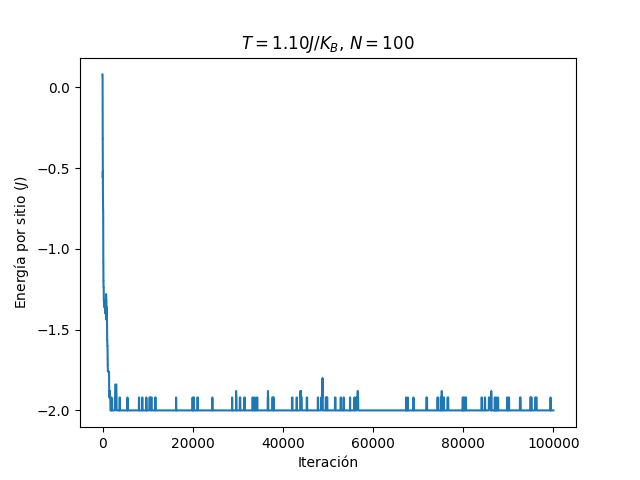
\includegraphics[width=\textwidth]{energia_200.png}
\end{subfigure}
\begin{subfigure}{0.7\textwidth}
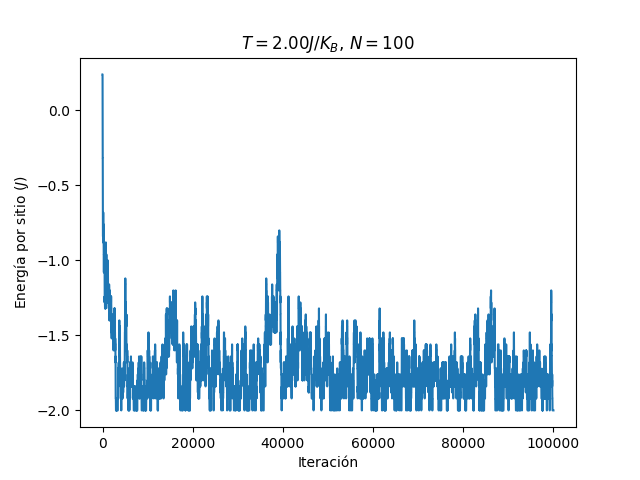
\includegraphics[width=\textwidth]{energia_500.png}
\end{subfigure}
\begin{subfigure}{0.7\textwidth}
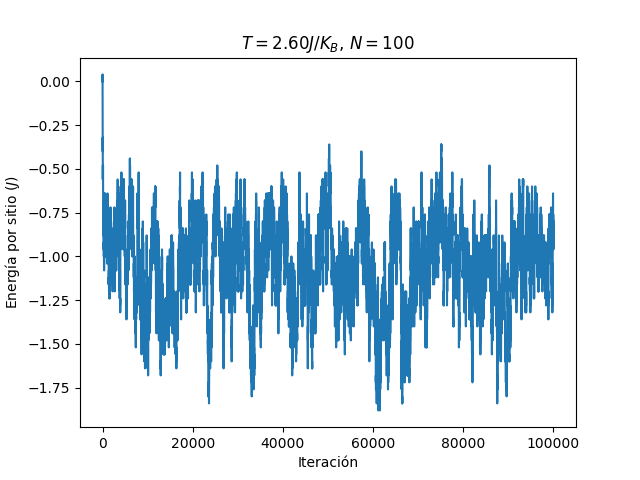
\includegraphics[width=\textwidth]{energia_700.png}
\end{subfigure}
\caption{\label{fig:energias}Se muestra la energía de la configuración obtenida en cada iteración para tres temperaturas distintas. En el título se indica la temperatura de la simulación $T$ y el número de espines considerados $N$.}
\end{figure}

Para hallar la curva de magnetización en función de temperatura en la figura \ref{fig:magnetizacion}, se barrieron 1000 temperaturas entre $0.5J/k_B$ y $3.5J/k_B$. Para cada temperatura la magnetización se calculó tomando la magnetización total en cada iteración y luego calculando el promedio descartando las primeras 10000 iteraciones. En la figura se observa que la magnetización se anula para temperaturas mayores a $2J/k_B$. Esto concuerda con la transición de fase hallada teóricamente en \eqref{ec:temperatura_critica}. Con esta figura podemos distinguir que a temperaturas menores que la crítica el sistema es magnético. En efecto, las fluctuaciones térmicas son bajas y la interacción en el Hamiltoniano hace que los espines apunten en la misma dirección (asumiendo $J>0$). Debido a esto, los momentos magnéticos en cada sitio contribuyen a la magnetización del material obteniendo así propiedades magnéticas. La transición de fase corresponde a que a altas temperaturas las fluctuaciones térmicas se vuelven más relevantes. En tal caso, la interacción entre espines se vuelve despreciable y estos toman posiciones aleatorias. De esta manera la contribución del momento magnético de cada sitio se vuelve destructiva y se anula la magnetización del material. 

\begin{figure}
\centering
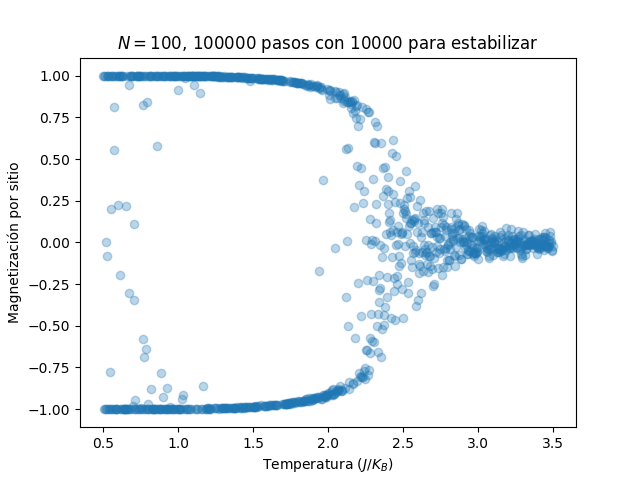
\includegraphics[width = 0.8\textwidth]{magnetizacion.png}
\caption{\label{fig:magnetizacion}Se muestra la magnetización por sitio en función de la temperatura.}
\end{figure}

La gráfica \ref{fig:energia} muestra como aumenta la energía promedio a medida que la temperatura sube. Esto es lo que se espera de nuestra noción intuitiva de la temperatura. Además, la suavidad de la curva muestra que en los 10000 pasos descartados sí se logra llegar al equilibrio, algo que debido a las fluctuaciones térmicas no se podía ver en las gráficas correspondientes a altas temperaturas en  \ref{fig:energias}.

\begin{figure}
\centering
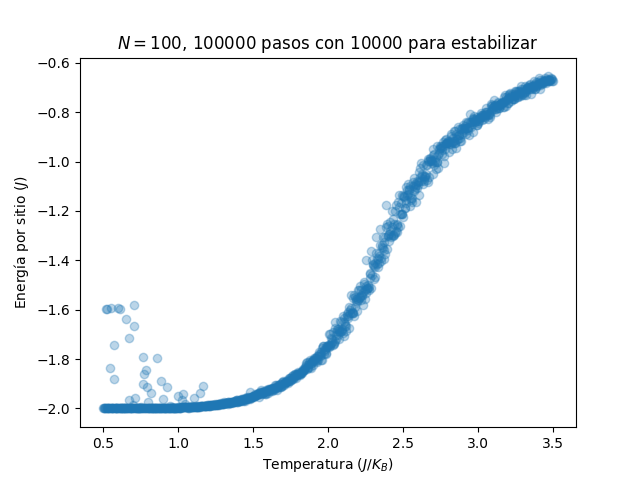
\includegraphics[width = 0.8\textwidth]{energia.png}
\caption{\label{fig:energia}Se muestra la energía promedio por sitio en función de la temperatura.}
\end{figure}

El código debidamente documentado fue
\lstinputlisting[language = Python, breaklines = True, showstringspaces = false, literate = {é}{{\'e}}1 {ó}{{\'o}}1 {í}{{\'i}}1]{ising.py}

\end{document}
